%	!Mode::"UTF-8"
%	本模板设置改自北京大学交叉学院 王宇哲学长和北京大学化学与分子工程学院 王应泽同学的分享,特此感谢!
%	模板制作:北京大学化学与分子工程学院 王梓涵
%	Email:2100011837@stu.pku.edu.cn
%	本模板仅适用于北京大学物理化学实验报告,其他学校请自行修改
%	吐槽:Latex用于写物化实验报告还是过于繁琐了,不过还是比Word好用多了(๑•̀ㅂ•́)و✧ (此吐槽由copilot自动生成,模板作者认为word更好用)
%	本模板仅供交流学习使用,不可用作商业用途。

\documentclass[12pt]{article}

%	页面设置
\usepackage{geometry}
\geometry{left=2.5cm, right=2.5cm, top=2.5cm, bottom=2.5cm}
\usepackage{graphicx}
\usepackage{ctex}
\usepackage{fontspec}
\usepackage{setspace}
\usepackage[usenames,dvipsnames]{xcolor}
\usepackage{titlesec}

%	字体设置
\setmainfont{Times New Roman}
\setCJKmainfont{SimSun}
\setCJKsansfont{SimHei}
\setCJKmainfont[AutoFakeBold=true]{SimSun}

%	表格设置\
\usepackage{array,colortbl}
\usepackage{makecell}
\newcommand{\addcell}[2][4]{\makecell{\zihao{#1}\textsf{#2}}}
\usepackage{titlesec}
\usepackage{booktabs}
\usepackage{ragged2e} 
\usepackage{multirow}
\usepackage{tabularx}

%	设置图注、表注
\usepackage{caption}
\usepackage{bicaption}
\captionsetup{labelsep=quad, font={small, bf}, skip=2pt}
\DeclareCaptionOption{english}[]{
    \renewcommand\figurename{Fig.}
    \renewcommand\tablename{Table}
}
\captionsetup[bi-second]{english}

%	设置页眉
\usepackage{fancyhdr}
\usepackage{xpatch}
\pagestyle{fancy}
\fancypagestyle{preContent}{
    	\fancyhead[L]{\zihao{-5} 物理化学实验}
    	\fancyhead[C]{\zihao{-5} 实验八\ \ 循环伏安法解析电极极化}
    	\fancyhead[R]{\zihao{-5} 2100011837\ 王梓涵}
		\renewcommand{\headrulewidth}{2pt}
		\renewcommand{\footrulewidth}{1pt}
		\xpretocmd\headrule{\color{BrickRed}}{}{\PatchFailed} % 设置页眉分割线颜色
		\xpretocmd\footrule{\color{BrickRed}}{}{\PatchFailed} % 设置页脚分割线颜色
}
\pagestyle{preContent}



%	设置首页页眉及取消首页页脚 若不需要首页页眉 请注释掉下列内容
\fancypagestyle{plain}{
	\fancyhead[L]{\zihao{-5} 物理化学实验}
    \fancyhead[C]{\zihao{-5} 实验八\ \ 循环伏安法解析电极极化}
	\fancyhead[R]{\zihao{-5} 2100011837\ 王梓涵}
	\cfoot{}
}

%	设置标题格式
\titleformat*{\section}{\color{Mahogany}\zihao{4}\sffamily}
\titleformat*{\subsection}{\zihao{-4}\sffamily}
\titleformat*{\subsubsection}{\zihao{-4}\sffamily}
\titlespacing*{\section}{0pt}{10pt}{10pt}
\titlespacing*{\subsection}{0pt}{10pt}{5pt}
\titlespacing*{\subsubsection}{0pt}{10pt}{5pt}


%	设置引用格式(ACS格式规范)
%	注意:请安装JabRef
%	JabRef使用参考:https://blog.csdn.net/weixin_44191286/article/details/85698921
\usepackage[super,round,comma,compress]{natbib}

%	数学公式增强
\usepackage{amsmath}
\usepackage{amssymb}

%	单位与数学式
\usepackage{siunitx}

%	设置封面
\begin{document}
    % 标题页
    \begin{titlepage}
    	% 页眉
    	\thispagestyle{plain}
        % 校徽图片
        \begin{figure}[h]
            \centering
            \includegraphics{pku.png}
        \end{figure}
        \vspace{24pt}
        % 标题
        \centerline{\zihao{-0} \textsf{\textcolor{Mahogany}{物理化学实验报告}}}
        \vspace{40pt} % 空行
        \begin{center}
            \begin{tabular}{cp{14.1cm}}
                % 题目
                \addcell[2]{题目:} & \addcell[2]{循环伏安法解析电极极化} \\
                \cline{2-2}
            \end{tabular}
        \end{center}
        \vspace{20pt} % 空行
        \begin{center}
            \doublespacing
            \begin{tabular}{cp{5cm}}
                % 姓名
                \addcell{姓\phantom{空格}名:\ } & \addcell{王梓涵} \\
                \cline{2-2}
                % 学号
                \addcell{学\phantom{空格}号:\ } & \addcell{2100011837}\\
                \cline{2-2}
                % 组别
                \addcell{组\phantom{空格}别:\ } & \addcell{22组} \\
                \cline{2-2}
                % 实验日期
                \addcell{实验日期:\ } & \addcell{2023.11.16}\\
                \cline{2-2}
                % 室温
                \addcell{室\phantom{空格}温:\ } & \addcell{293.82\ K}\\
                \cline{2-2}
                % 大气压强
                \addcell{大气压强:\ } & \addcell{101.78\ kPa}\\
                \cline{2-2}
            \end{tabular}
            \begin{tabular*}{\textwidth}{c}
                \\ % 这是空行
                \\ % 这是空行
                \\ % 这是空行
                \hline % 分割线
            \end{tabular*}
        \end{center}
        % 摘要
        \textsf{\textcolor{BrickRed}{摘\ \ 要}}\ \ 本实验利用循环伏安法研究了硫酸水溶液中Pt电极表面的氧还原反应和甲醇氧化反应,并测定了Pt电极表面的活性面积。经计算得到铂电极电化学活性面积$S=0.020\ \ {\rm cm^{2}}$,并读出氧气的起始还原电位为$0.48\ \ {\rm V}$。绘制了有无甲醇存在时扫速为0.1 V/s的氮气饱和的0.05 M 硫酸溶液的CV曲线,确定了甲醇的起始氧化电位为$0.03\ \ {\rm V}$。绘制了直接甲醇燃料电池的$U-P$曲线,工作电压为$0.18\ \ {\rm V}$时达到最大输出功率$3.5\times 10^{-7}\ \ {\rm W}$。
        \\
        \\
        % 关键字
        \textsf{\textcolor{BrickRed}{关键词}}\ \ 循环伏安法;ORR;MOR;甲醇燃料电池
    \end{titlepage}

    \section{引言}
		\subsection{实验目的}
			本实验的实验目的主要有以下几点\cite{physchemlab}:\par
			\ \ \ \ \ \ \ \ 1. 了解应用循环伏安法获得电极极化信息的方法。\par
			\ \ \ \ \ \ \ \	2. 学会分析电流-电势曲线,以及铂电极电化学活性面积的测算方法。\par
			\ \ \ \ \ \ \ \	3. 了解扫描速度、气氛以及电极表面状态对电流-电势曲线的影响。\par
		\subsection{实验原理和实验方法}
		本实验的实验原理和实验方法在实验预习报告中如\textbf{图1}所示: \par
		\begin{figure}[h]
			\centering
			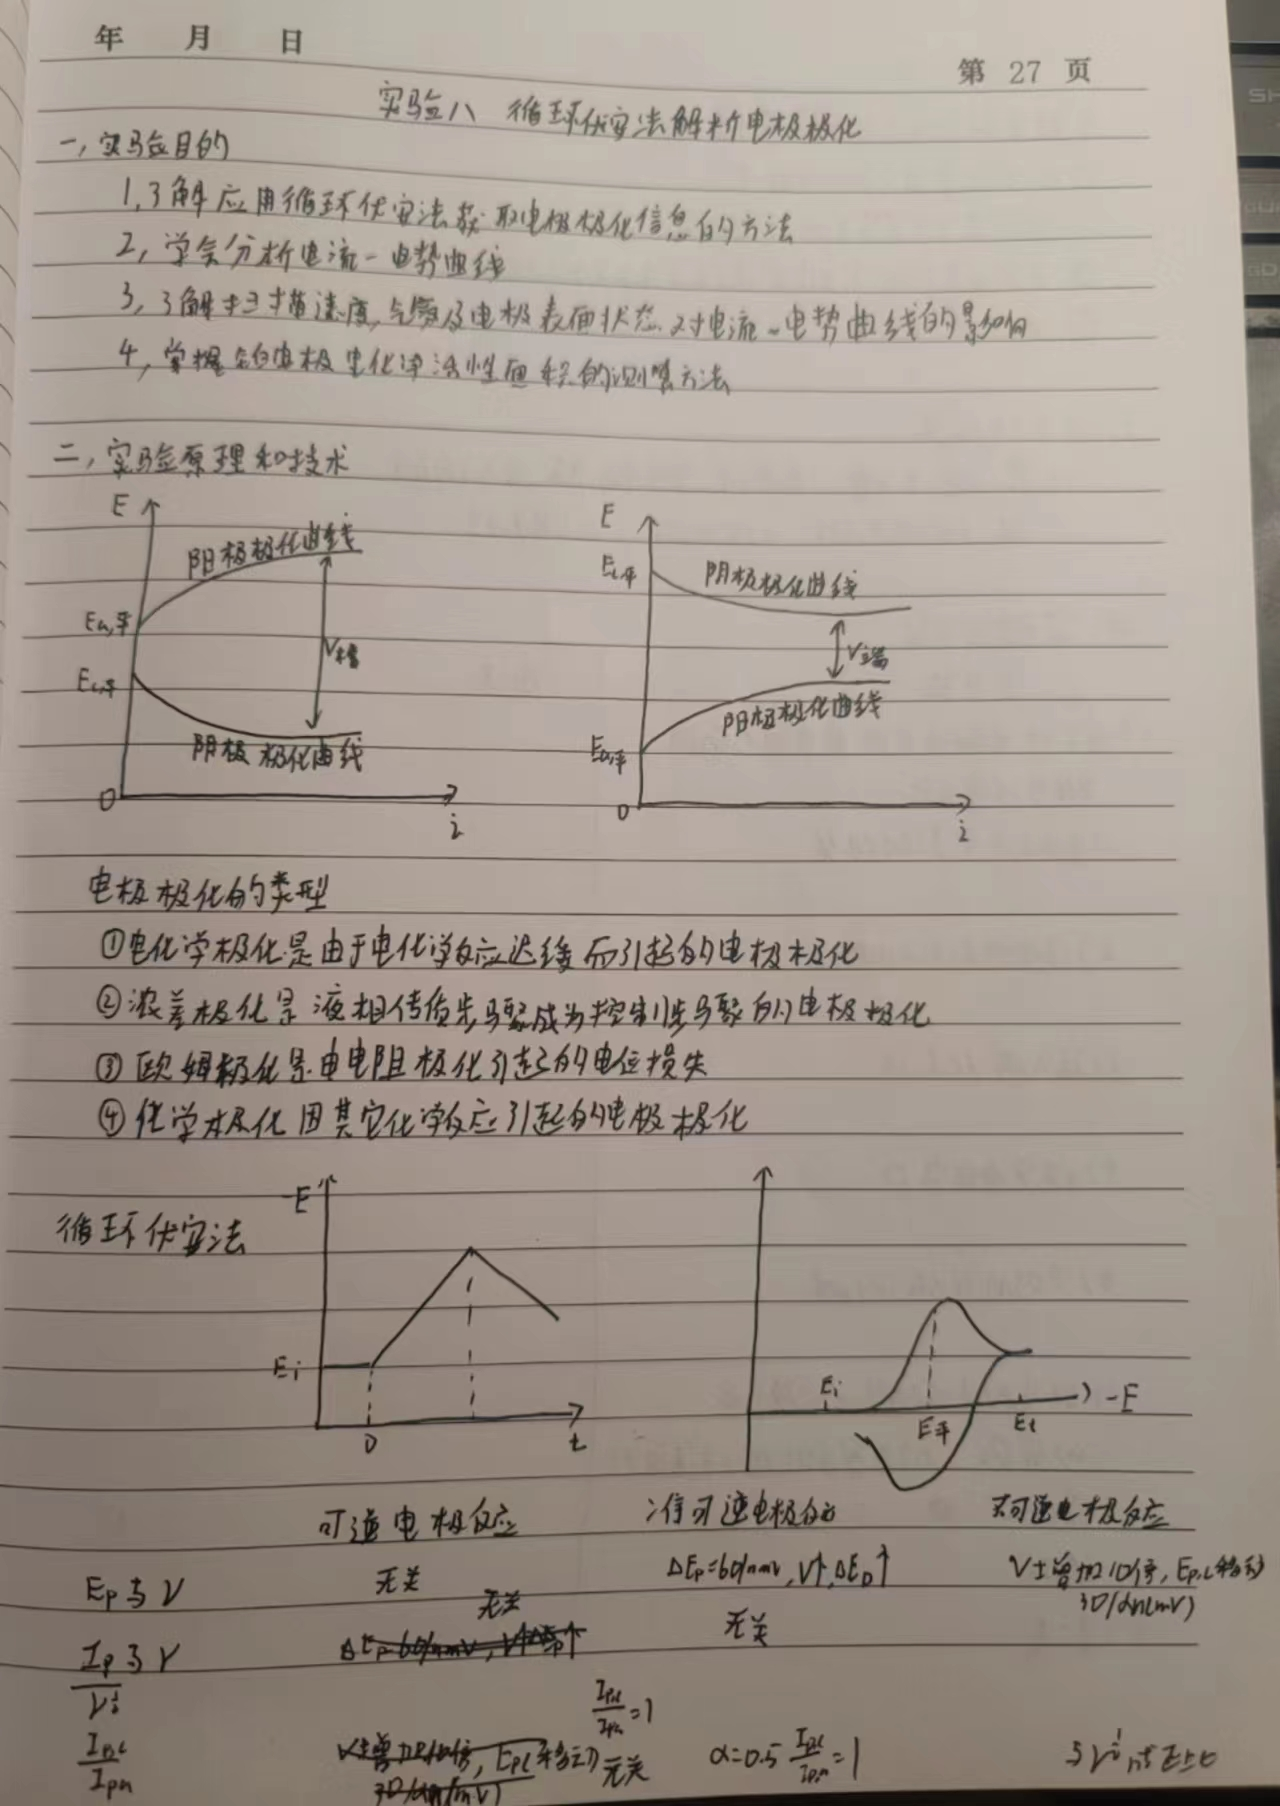
\includegraphics[width=0.6\textwidth]{1.png}
			\bicaption{实验预习报告的实验原理部分}{The principle part of the experiment in the experiment preview report}
		\end{figure}
			
	     
    \section{实验部分}
    	\subsection{仪器和试剂}
    		仪器:\ \ 三电极电解池,CHI电化学工作站,磁力搅拌恒温槽,温度计,氧气钢瓶,氮气钢瓶,工作电极(W.E.)——铂圆盘电极,辅助电极(C.E.)——铂片电极,参比电极(R.E.)——双盐桥饱和甘汞电极。\par
			试剂:\ \  电解质:$0.05\ \ {\rm M}$硫酸水溶液,$0.1\ \ {\rm M}$硫酸水溶液,$0.1\ \ {\rm M}$甲醇水溶液,去离子水。\par 
    			
    	\subsection{实验内容}
		 本实验的实验操作如下所示,其中笔者的思考和具体实验中的不同操作会在括号中写出。\par
		\subsubsection{电极的清洗及组装}
			将三电极电解池与电化学工作站相连:工作电极铂圆盘电极与绿线相连,辅助电极铂片电极与红线相连,参比电极双盐桥饱和甘汞电极与白线相连。三电极法实验装置如\textbf{图2}所示。\par
			用去离子水清洗电极系统和电解池,并向参比电极的二次盐桥与电解池中加入适量$0.05 \ \ {\rm M}$硫酸溶液。通入$\rm N_{2}$赶走电解质溶液中的残余$\rm O_{2}$直至饱和。\par
			 \begin{figure}[!h]
				\centering
				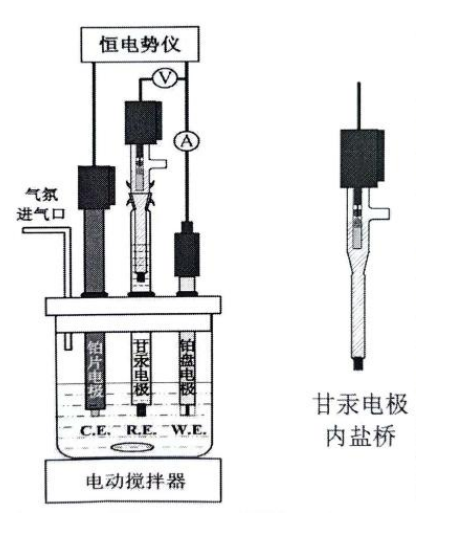
\includegraphics[width=0.5\textwidth]{2.png}
				\bicaption{三电极法实验装置}{Three electrode method experimental device}
			\end{figure}
		\subsubsection{测试并确定电位窗口}
			调整电位窗口,使得在电位窗口内水不发生电解,同时包含所要研究的电化学信息,确定电位窗口为$-0.31\sim 1.2\ \ {\rm V}$。\par
		\subsubsection{电化学清洁和活化电极}
		 	用CV法清洁活化电极,电势扫描范围$-0.31\rm{V}\sim 1.3\rm{V}$,以$0.5\ \ {\rm V\cdot s^{-1}}$的扫速扫描$500$个周期,观察CV曲线形状基本保持不变后停止活化。\textbf{(这里需要注意若通入氮气量不足,体系可能会在为完全排出氧气的情况下达到平衡,因此电极活化和清洁需要耐心等待一段时间)}\par
		\subsubsection{空白实验}
			在$\rm N_{2}$饱和下测量CV,测定不同扫描速度$0.5\ \ {\rm V\cdot s^{-1}}$、$0.2\ \ {\rm V\cdot s^{-1}}$、$0.1\ \ {\rm V\cdot s^{-1}}$下的CV曲线。\par
		\subsubsection{铂电极表面的氧还原反应}
			向电解池内通入$\rm O_{2}$至饱和,设定扫描速度为$0.1\ \ {\rm V\cdot s^{-1}}$,考察不同搅拌速度对氧还原反应的影响,分别测定快速搅拌(通气并开搅拌)、低速搅拌(停搅拌仅通气)、电解质静止(停搅拌不通气)条件下的CV曲线。\textbf{(这里要注意通气与搅拌速度不能过快,若速度过快则会使得所得曲线极其不稳定)}\par
		\subsubsection{铂电极表面的甲醇电化学氧化反应}
			将$0.1\ \ {\rm M}$硫酸水溶液与$0.1\ \ {\rm M}$甲醇水溶液等体积混合加入电解池,通入$\rm N_{2}$排除溶液中残余的空气,设定扫描速度为$0.1\ \ {\rm V\cdot s^{-1}}$,测定CV曲线。\textbf{(一定要等待氮气将氧气全部排出,不然会对数据造成较大影响)}\par
		\subsubsection{清洁电解池和电极}
			用去离子水清洗电解池和电极,测量$\rm N_{2}$氛围下$0.05\ \ {\rm M}$硫酸溶液中的CV曲线,与实验开始时相同条件测量的曲线一致后,由老师确认,将实验仪器复原到初始状态,并电解池内更换为去离子水。\par

	 \section{数据与结果}
 		\subsection{实验数据记录及处理}
 			\subsubsection{不同扫描速度下的 CV 曲线}
			 测定不同扫描速度下的CV曲线,为便于观察仅示出第$9\sim 10$个segment,结果如\textbf{图3}所示,蓝色曲线、红色曲线、棕色曲线分别为$0.5\ \ {\rm V\cdot s^{-1}}$、$0.2\ \ {\rm V\cdot s^{-1}}$、$0.1\ \ {\rm V\cdot s^{-1}}$下的CV曲线。
		 	\begin{figure}[h]
				\centering
				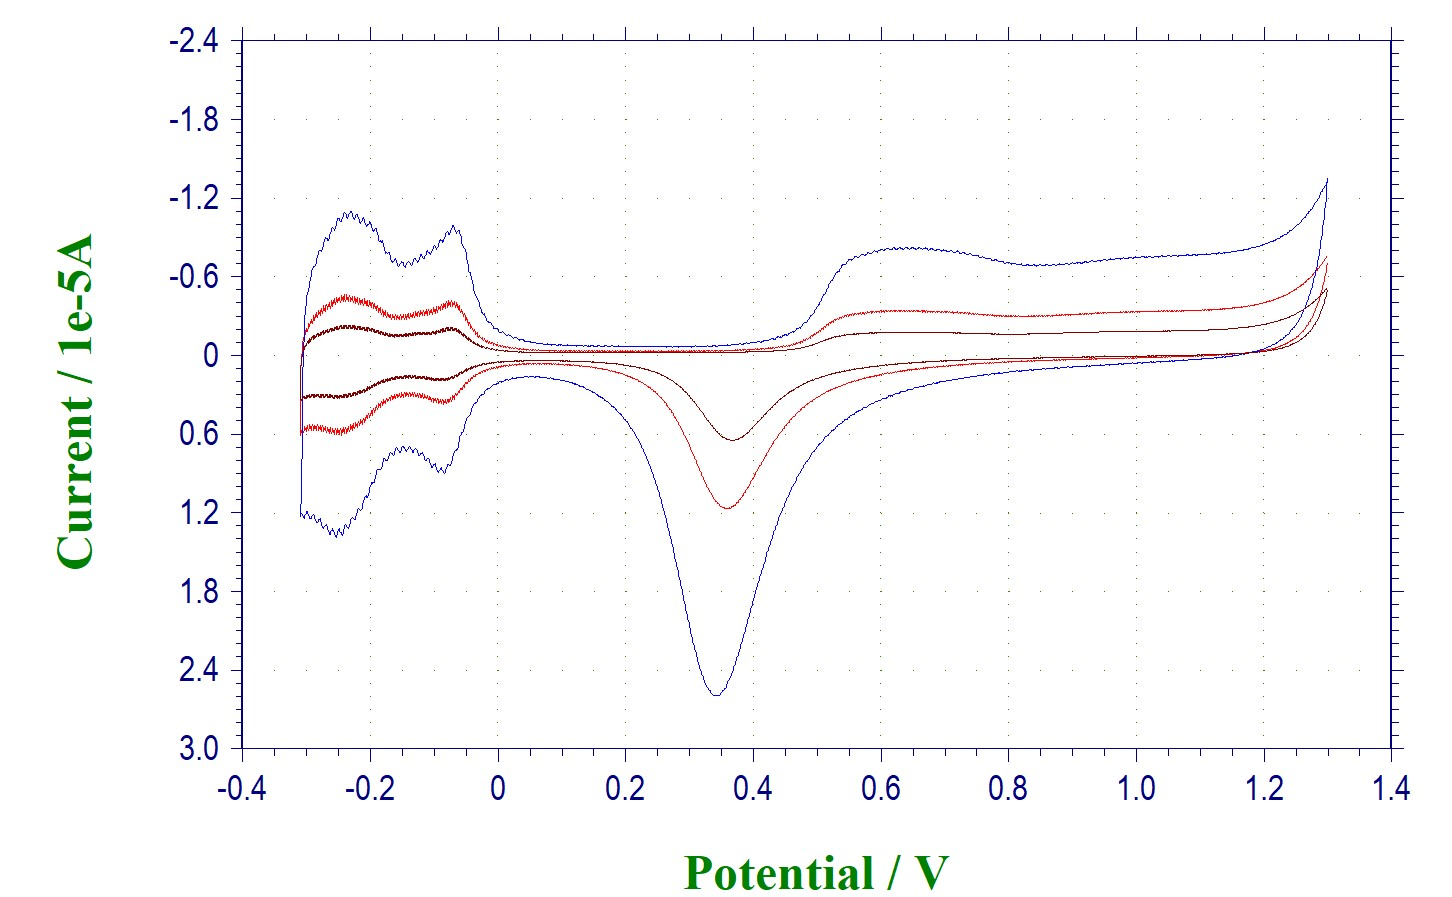
\includegraphics[width=0.7\textwidth]{3.png}
				\bicaption{不同扫描速度下的CV曲线}{CV curve under different scanning speed}
			\end{figure}
			\par
			从\textbf{图3}可以看出,不同扫描速度下,峰电位位置基本不变,但扫描速度越大峰电流越大,这与循环伏安法的原理是相符的。根据Randles–Ševčík方程,峰电流$i_{p}$满足
			$$
			i_{p}=0.4463 n F A C\sqrt{\frac{nFvD}{RT}}\propto\sqrt{v}
			$$
			$v$为扫描速度。因此,峰电流$i_{p}$随扫描速度$v$的增大而增大,这与观察到的实验现象一致。\par
			同时我们可以注意到,图中左侧(氢区)的对称性较好,说明氢脱附-吸附反应的可逆性好;而右侧(氧区)的对称性较差,只有明显的含氧物种还原峰,在0.45V左右,观察不到对应的氧化峰,说明此反应的可逆性较差。
			\subsubsection{铂电极的电化学活性面积}
			利用氮气饱和的硫酸溶液中铂电极的CV曲线中氢原子脱附峰的电量求算铂电极的电化学活性面积。取扫描速度为$0.1\ \ {\rm V\cdot s^{-1}}$下的CV曲线第9个segment的实验数据,根据扫描速度,将原始数据的横坐标电势$\varphi$换算成时间$t$,以双电层电位作为基线,使用Origin对氢原子脱附峰峰面积进行积分,得到氢原子脱附峰的电量,结果如\textbf{图4}所示,图中灰色区域为积分区域。\par
			\begin{figure}[h]
				\centering
				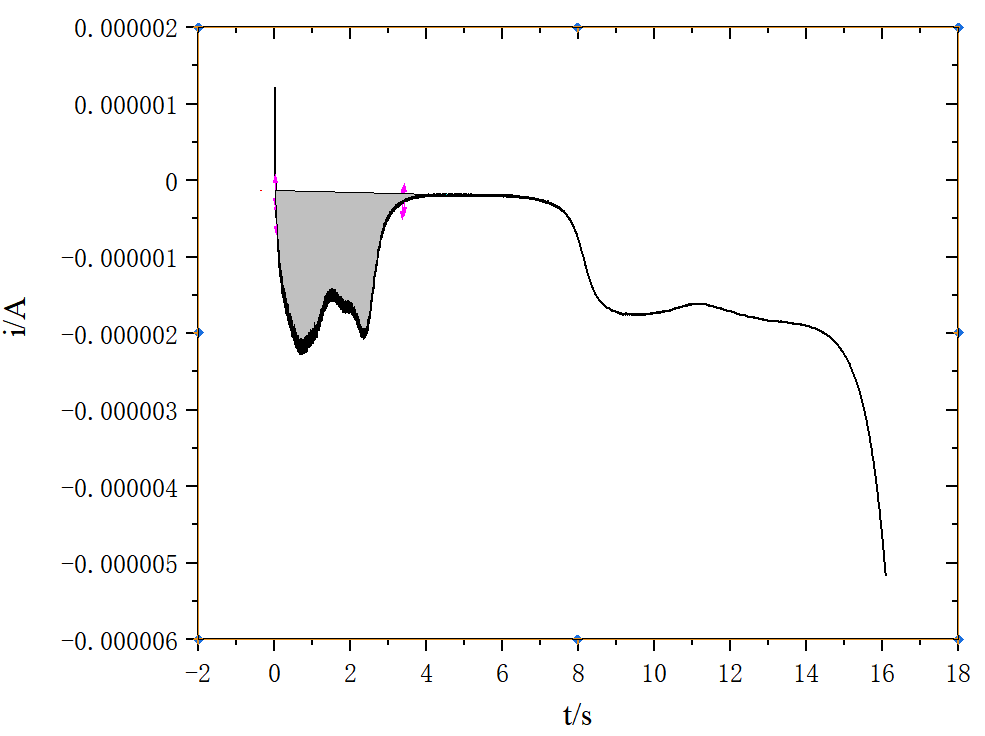
\includegraphics[width=0.7\textwidth]{4.png}
				\bicaption{由铂电极CV曲线积分求氢原子脱附峰电量}{H desorption peak electricity calculation by integrating the CV curve of Pt electrode}
			\end{figure}
			\par
			根据\textbf{图4},可计算得到铂电极表面单层氢原子脱附的电量:
			$$
			q=\int i dt= \int \frac{i}{v}d{\rm E}= 4.26\times10^{-6}\ \ {\rm C}
			$$
			\par
			查阅资料\citealp{physchemlab}可知多晶Pt表面满单层氢脱附的电量为$0.21\ \ {\rm mC\cdot m^{-2}}$,采用该数据进行计算,则实验使用的铂电极电化学活性面积:
			$$
			S=\frac{4.26\times10^{-6}\ \ {\rm C}}{0.21\ \ {\rm mC\cdot cm^{-2}}}=0.020\ \ {\rm cm^{2}}
			$$


			\subsubsection{铂电极表面的氧还原反应}
			测定不同搅拌速度下氧还原反应的CV曲线,为便于观察仅示出1个segment(即为线性扫描曲线LSV),结果如\textbf{图5}所示,图中O2-快(棕色曲线)、O2-慢(绿色曲线)、O2-静(红色曲线),空白-01(蓝色曲线)分别为快速搅拌、低速搅拌、电解质静止,以及未氧气饱和下的LSV曲线。\par
			\begin{figure}[h]
				\centering
				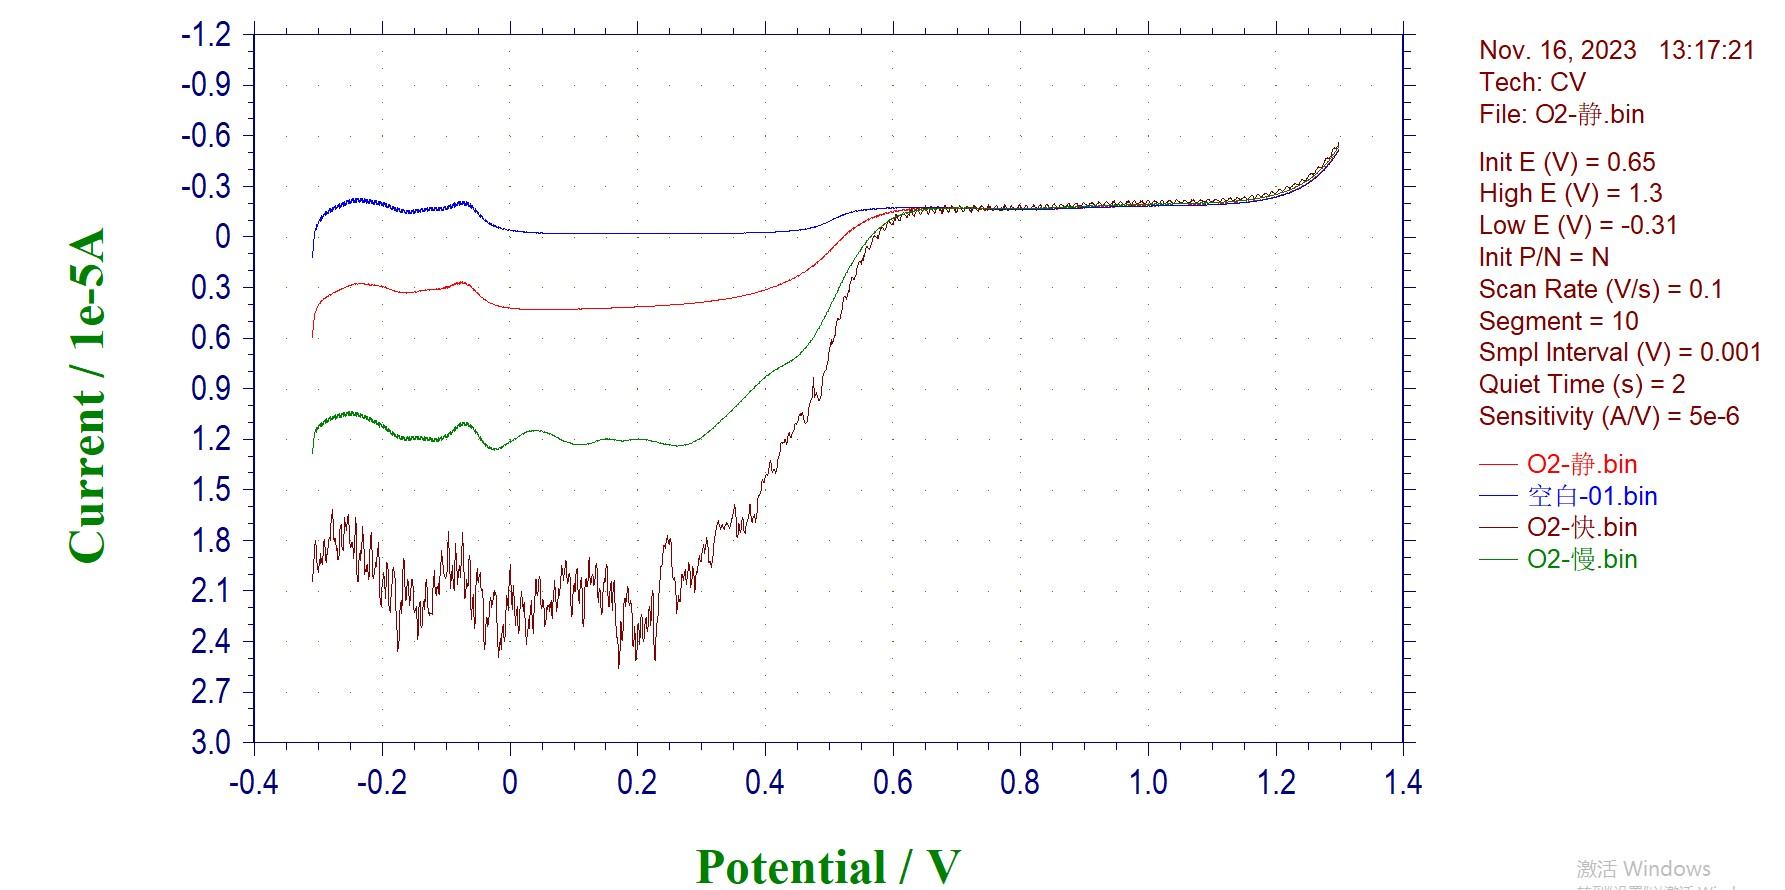
\includegraphics[width=0.85\textwidth]{5.png}
				\bicaption{不同搅拌速度下氧还原反应的LSV曲线}{LSV curve of oxygen reduction reaction under different stirring speed}
			\end{figure}
			\par
			从\textbf{图5}可以看出,不同搅拌速度下氧还原反应的LSV曲线走势大致相同,对于不涉及氧还原反应的部分(电势高于$\sim0.45{\rm V}$),不同搅拌速度下的LSV曲线基本重合;而对于电势较低的氧还原电势区(电势低于$\sim 0.4{\rm V}$),搅拌越剧烈,氧还原的峰电流$i_{p}$越大,并且LSV曲线的波动越显著;这是由于在搅拌速度较快时,物质传输速度快,铂电极附近消耗的$\rm O_{2}$和$\rm H^{+}$能得到及时补充,浓度更大,因此氧还原的峰电流$i_{p}$较大;但由于搅拌速度较快时对铂电极附近溶液产生较大扰动,$\rm O_{2}$、$\rm H^{+}$浓度变化剧烈,导致快速搅拌的LSV曲线产生显著波动。\par
			对比扫描速度为$0.1\ \ {\rm V\cdot s^{-1}}$、$\rm N_{2}$饱和的硫酸溶液中铂电极的CV曲线和扫描速度为$0.1\ \ {\rm V\cdot s^{-1}}$、电解质静止、$\rm O_{2}$饱和的硫酸溶液中氧还原反应的CV曲线,为便于观察仅示出第$9\sim 10$个segment,如\textbf{图6}所示,图中空白-01(蓝色曲线)、O2-静(红色曲线)分别为氮气饱和与氧气饱和的硫酸溶液中的CV曲线。
			\begin{figure}[h]
				\centering
				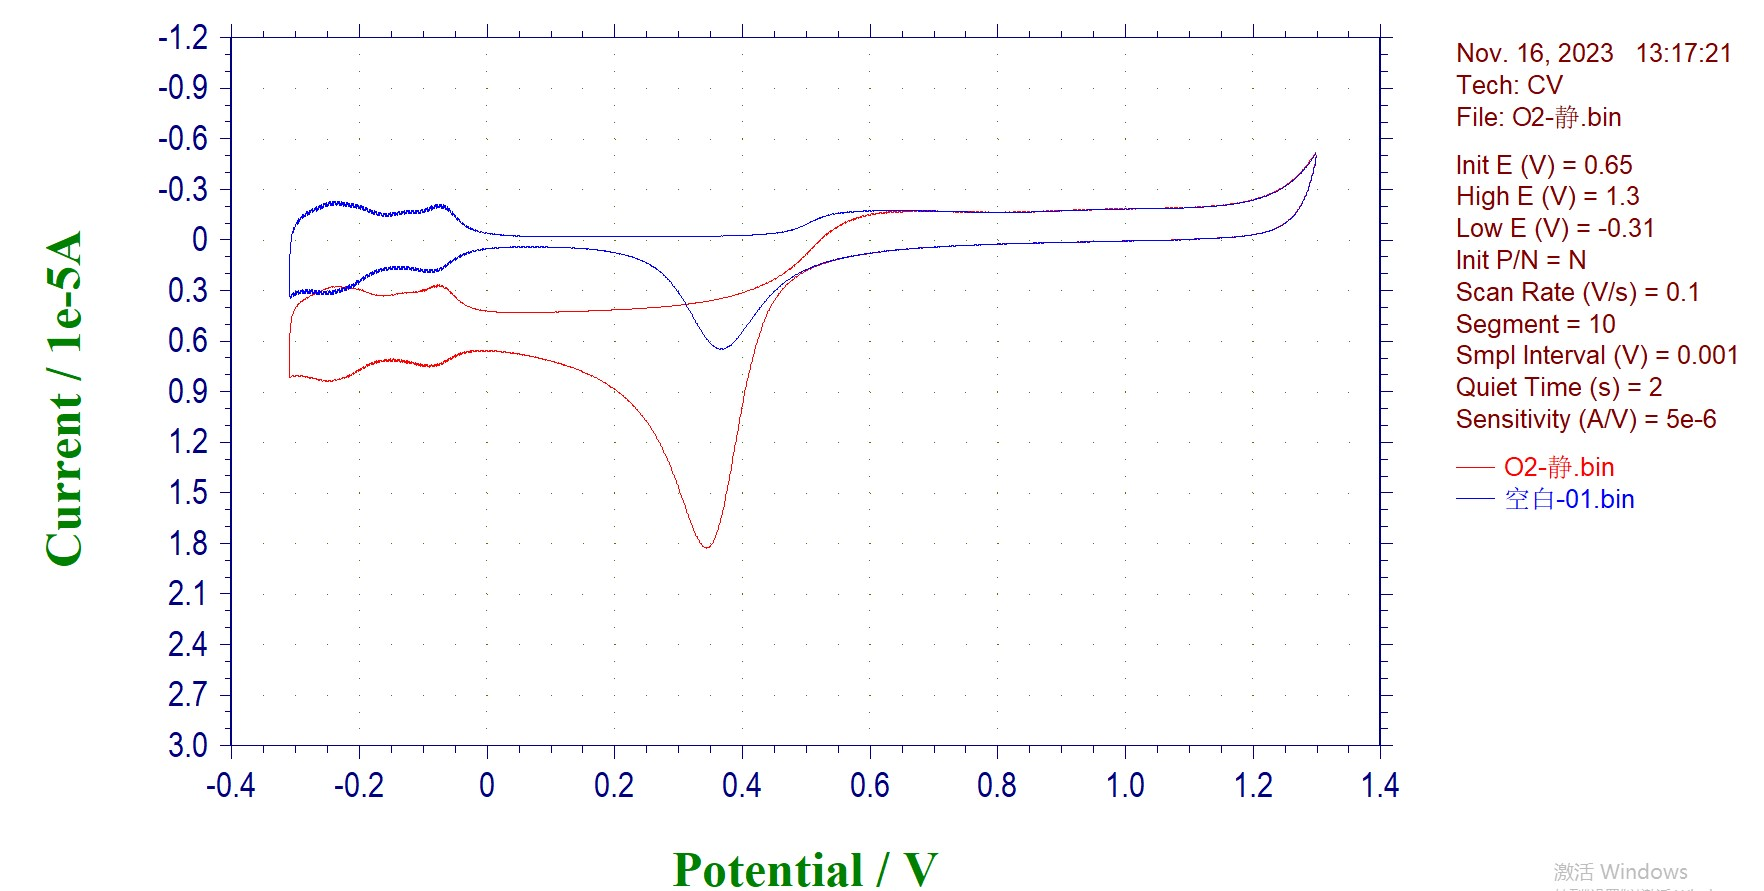
\includegraphics[width=0.85\textwidth]{6.png}
				\bicaption{氮气与氧气饱和的硫酸溶液中的CV曲线}{CV curve in sulfuric acid solution saturated with nitrogen and oxygen}
			\end{figure}
			\par
			根据\textbf{图6},读出电势升高过程中含氧物种吸附氧化的起始氧化电位$\rm{E_{ORR}}=0.65\ \ {\rm V}$,电势降低过程中氧气的起始还原电位为$0.48\ \ {\rm V}$。故若以起始还原电位为基准,氧化过程中氧的过电势:
			$$
			\eta_{\rm O}=(0.66-0.48)\ \ {\rm V}=0.18\ \ {\rm V}
			$$
			\par
			推测该过电势$\eta_{\rm O}$的形成是由于含氧物种吸附氧化过程中,氧气在铂电极表面析出的电化学反应迟缓,造成了电化学极化。\par
			
			\subsubsection{铂电极表面的甲醇电化学氧化反应}
			测定铂电极表面甲醇电化学氧化反应的CV曲线,为便于观察仅示出第$9\sim 10$个segment,结果如\textbf{图4}所示,图中蓝色曲线、红色曲线分别为硫酸溶液中铂电极表面甲醇电化学氧化与氮气饱和的CV曲线。
			\begin{figure}[h]
				\centering
				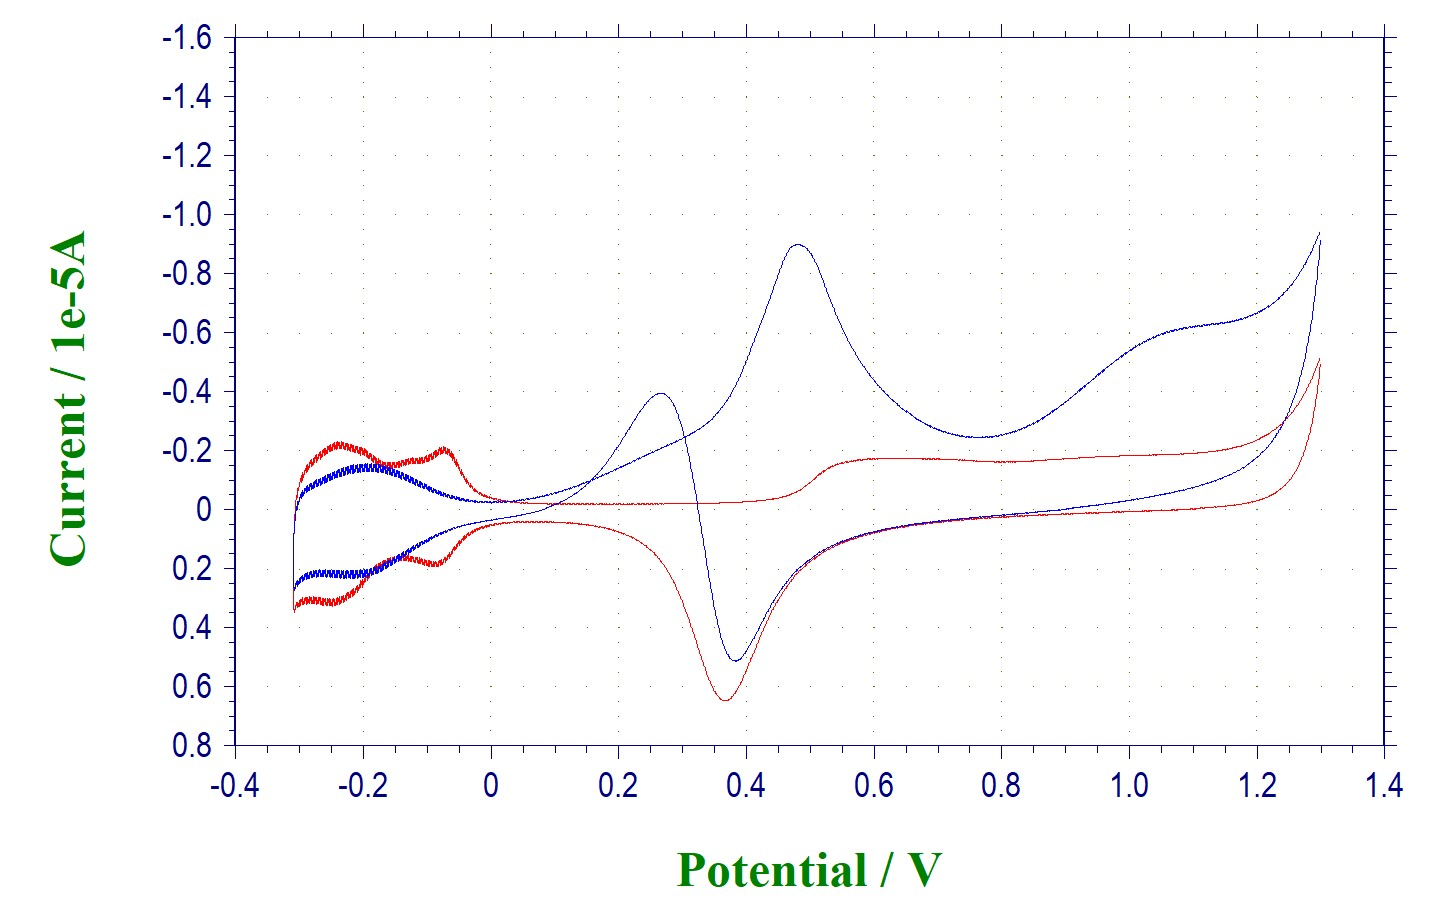
\includegraphics[width=0.8\textwidth]{7.png}
				\bicaption{硫酸溶液中甲醇氧化与氮气饱和的CV曲线}{CV curve of methanol oxidation and nitrogen saturation in sulfuric acid solution}
			\end{figure}
			\par
			根据\textbf{图7},读出甲醇的起始氧化电位$\rm{E_{MOR}}= 0.03\ \ {\rm V}$。

			\subsubsection{甲醇燃料电池输出电压-输出功率曲线}
			直接甲醇燃料电池(DMFC)中负极为甲醇失去电子溶液,正极为氧气得电子,因而等效于本实验中3.13的下半段和3.14上半段相叠加。扣除扫速氮气饱和的CV曲线背景后,取MOR正支(电流取相反数),和ORR负支,叠加作\textbf{图8}
			\begin{figure}[h]
				\centering
				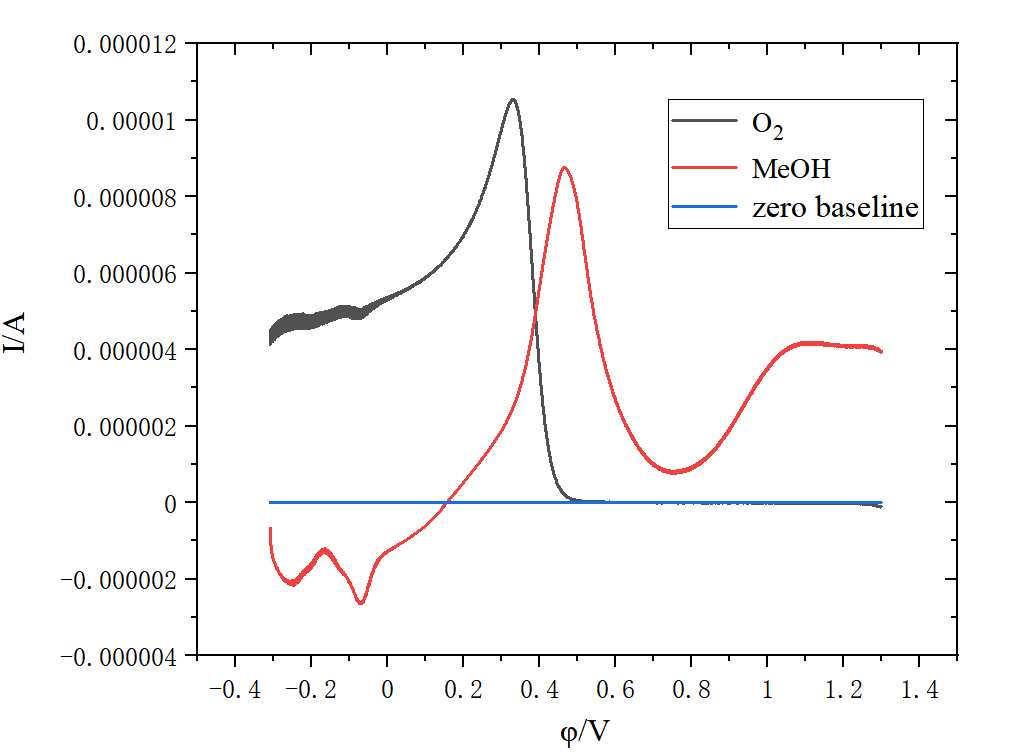
\includegraphics[width=0.8\textwidth]{8.png}
				\bicaption{直接甲醇燃料电池阳极、阴极$\varphi-i$工作曲线}{$\varphi-i$ working curve of anode and cathode of direct methanol fuel cell}
			\end{figure}
			\par
			图中两条曲线与zero baseline围成的区域即为电池可以工作的区域,此时ORR电势大于MOR电势,且电势差处于水的稳定区。
			在直接甲醇燃料电池中,在一定的工作电流$i$下,阳极(负极,甲醇氧化)电势$\varphi_{a}$
			低于阴极(正极,氧气还原)电势$\varphi_{c}$。在\textbf{图8}中选取$i$相同时$\varphi_{a}<\varphi_{c}$的部分,作一组平行于$\varphi$轴的直线与两条曲线相交,读取交点坐标对应的电势$\varphi_{a}$、$\varphi_{c}$,计算两极电势差:
			$$
			U=\varphi_{c}-\varphi_{a}
			$$
			即为直接甲醇燃料电池的输出电压,根据
			$$
			P=Ui
			$$
			计算直接甲醇燃料电池的输出功率$P$。以上各项数据示于\textbf{表1}。
			\begin{table}[h]
				\centering
				\arrayrulecolor{Maroon}
				\zihao{5}
				\bicaption{直接甲醇燃料电池的两极电势、输出电压和输出功率}{Polar potential, output voltage and output power of direct methanol fuel cell}
				\begin{tabular}{ccccc}
					\toprule
					$i/{\rm 10^{-6}\ \ A}$ & $\varphi_{a}/{\rm V}$ & $\varphi_{c}/{\rm V}$ & $U/{\rm V}$ & $P/{\rm 10^{-6}\ \ W}$ \\
					\midrule
				1.00 & 0.213 & 0.485 & 0.272 & 0.272 \\
				1.50 & 0.259 & 0.477 & 0.218 & 0.327 \\
				2.00 & 0.288 & 0.462 & 0.174 & 0.348 \\
				2.50 & 0.322 & 0.456 & 0.134 & 0.335 \\
				3.00 & 0.344 & 0.448 & 0.104 & 0.312 \\
				3.50 & 0.369 & 0.445 & 0.076 & 0.266 \\
				4.00 & 0.379 & 0.437 & 0.058 & 0.232 \\
					\bottomrule
				\end{tabular}
			\end{table}
			\par
			根据\textbf{表1}数据,作出直接甲醇燃料电池的输出电压$U$-输出功率$P$曲线,如\textbf{图9}所示。
			\begin{figure}[h]
				\centering
				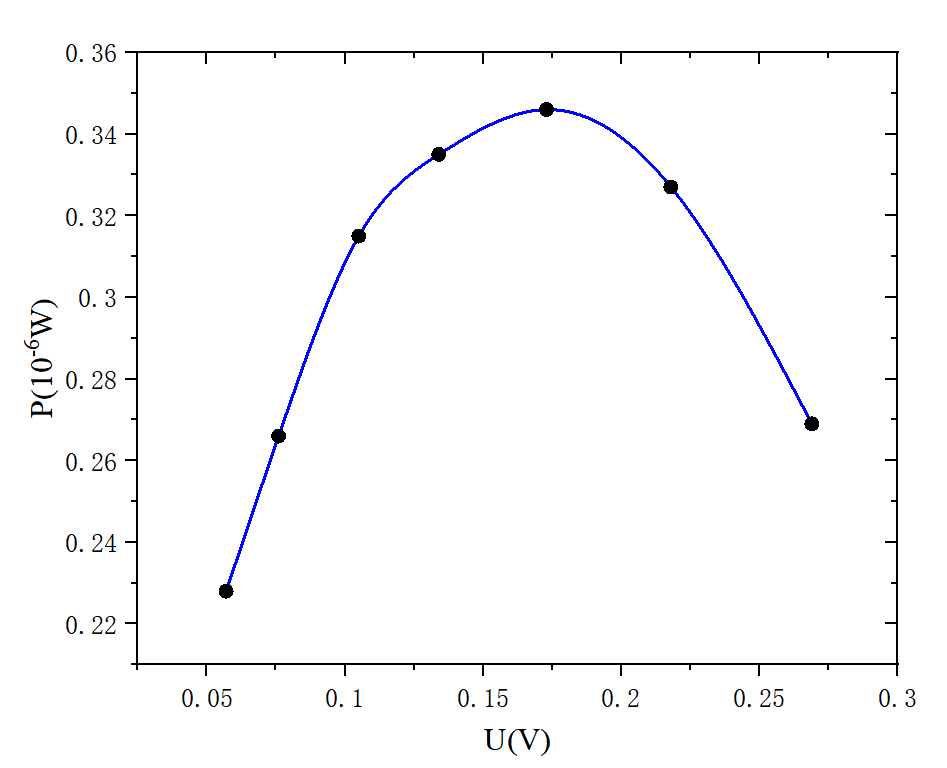
\includegraphics[width=0.8\textwidth]{9.png}
				\bicaption{直接甲醇燃料电池$U-P$曲线}{$U-P$ curve of direct methanol fuel cell}
			\end{figure}
			\par
			根据\textbf{图9}可以看出,直接甲醇燃料电池的输出功率$P$随输出电压$U$的增大而先增大后减小,$U\approx0.18\ \ {\rm V}$时输出功率达最大值,$P_{max}\approx 3.5\times10^{-7}\ \ {\rm W}$。

	\section{讨论与结论}
	 \subsection{实验误差}
	 本实验每个步骤都存在可能引入误差的地方,下面将对其进行分别分析。\par
		\subsubsection{测定铂电极电化学活性面积}
		\begin{enumerate}
			\item \textbf{电极极化}:因为电极极化,氢原子脱附的实际电量与根据CV曲线测算的电量并不严格相等,有一部分电子转移过程中的电量损耗,CV曲线积分得到的电量大于实际氢原子脱附的电量,导致测算的铂电极电化学活性面积偏大。
			\item \textbf{浓差极化}:受到迁移速率的限制,氢的吸附和脱附过程可能进行不完全。可能氢尚未充分吸附到铂电极表面时,扫描已经反向,开始脱附过程,导致氢原子未能充分占据铂电极表面的全部活性位点,测算的铂电极电化学活性面积偏小。
		\end{enumerate}
		\subsubsection{直接甲醇燃料电池$U-P$曲线的误差分析}
		\begin{enumerate}
			\item \textbf{甲醇测量时为充分脱氧}:在测量甲醇前通入氮气排除氧气的过程可能进行的不完全,导致甲醇电化学氧化的 CV 曲线测定不够准确,根据\textbf{图8} 可以看出,甲醇氧化的双电层区有一定程度的上抬,在氢区与${\rm N_{2}}$的曲线不重合,导致在扣除背景时出现一定的偏差,从而导致甲醇氧化的 CV 曲线不够准确。
		\end{enumerate}
	
 		\subsection{实验结论}
		 本实验利用循环伏安法研究了硫酸水溶液中Pt电极表面的氧还原反应和甲醇氧化反应,并测定了Pt电极表面的活性面积,计算得到铂电极电化学活性面积$S=0.020\ \ {\rm cm^{2}}$,并读出氧气的起始还原电位为$0.48\ \ {\rm V}$。绘制了有无甲醇存在时扫速为0.1 V/s的氮气饱和的0.05 M 硫酸溶液的CV曲线,确定了甲醇的起始氧化电位为$0.03\ \ {\rm V}$。绘制了直接甲醇燃料电池的$U-P$曲线,工作电压为$0.18\ \ {\rm V}$时达到最大输出功率$3.5\times 10^{-7}\ \ {\rm W}$。
		 

\vbox{}  
%参考文献
\bibliographystyle{unsrt}
\bibliography{cite}
\end{document}